\documentclass[a4paper, 12pt]{article}
\usepackage{graphicx} % Required for inserting images
\graphicspath{{./images/}}
\usepackage{float}  % For [H] option to control figure placement

\title{Crop Yield Predictor}
\author{297845 \\ University of Sussex}
\date{May 2025}

\begin{document}

\maketitle

\listoffigures     % Table of Figures


\section{Performance}
\subsection{Performance Metrics}
To measure the performance of the trained multi layer perceptron model, a combination of distance based and correlation based metrics were used. The selected metrics provide a multi dimensional view of model accuracy and generalization:

1. Root Mean Squared Error (RMSE): Measures the square root of the average squared differences between predicted and actual values. It penalizes large errors more heavily than MAE and retains the same unit as the target variable.

2. Mean Absolute Error (MAE): Represents the average magnitude of the absolute errors in a set of predictions.

3. R squared ($R^2$): The proportion of the variance in the dependent variable that is predictable from the independent variables.

These metrics were computed on a held out on the test set, which consisted of crop yield data for all countries over the years of only 2021 and 2022.

The final results on the test set were as follows:

$RMSE: 22,475$

$MAE: 15,131$

$R^2$ Score: $0.9882$

The relatively low RMSE and MAE error values suggest that the model makes small errors in prediction on average. An $R^2$ value of 0.98 indicates that the model explains most of the portion of the variance in the output variable, which is the crop yield for each country, which further validates the model’s consistency.

The $R^2$ score starts with a value of -2.5 at 0 epoch, then reaches 0 after only 10 epochs, and then it reaches a value of 0.5 after just approximately 20 epochs. Then the $R^2$ score reaches approximately one at the end of the training phase, after 100 epochs, as can be seen in Figure \ref{fig:1}.

\begin{figure}[H]
    \centering
    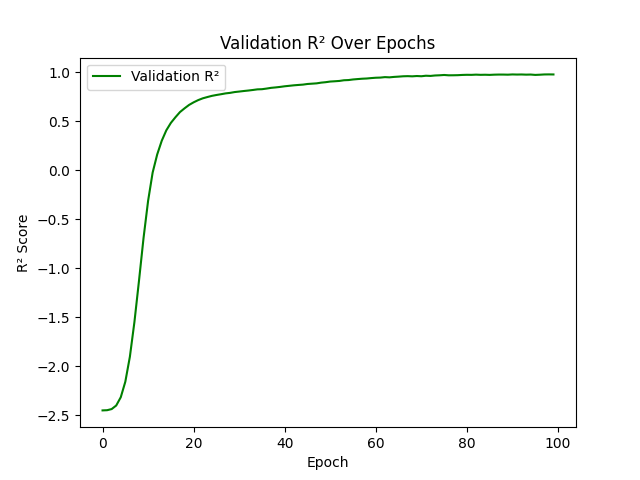
\includegraphics[width=1\linewidth]{val_r2.png}
    \caption{$R^2$ score Vs No. of Epochs}
    \label{fig:1}
\end{figure}

The RMSE starts with a value of 380,000 at 0 epoch, then reaches 100,000 after only 20 epochs,. Then the RMSE falls just below 50,000 at the end of the training phase, after 100 epochs, as can be seen in Figure \ref{fig:2}.

\begin{figure}[H]
    \centering
    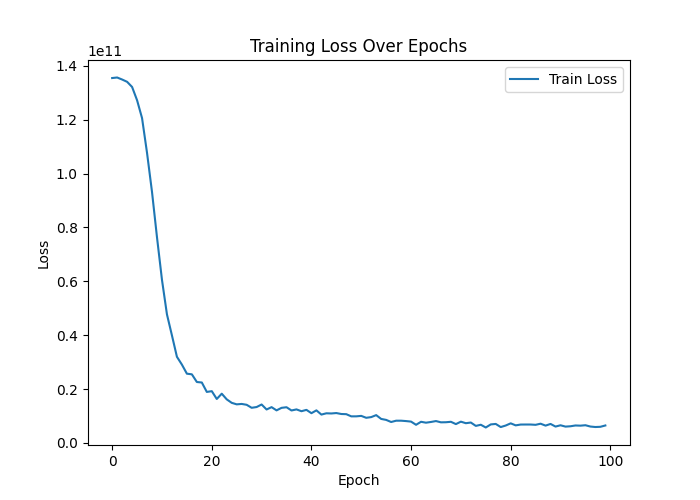
\includegraphics[width=1\linewidth]{training_loss.png}
    \caption{RMSE Vs No. of Epochs}
    \label{fig:2}
\end{figure}

The training loss exhibited a rapid decrease in the initial epochs, plummeting from approximately $1.35×10^{11}$ to around $10^{11}$ within the first 10 epochs. This steep decline suggests that the model quickly learned significant patterns in the training data during this phase. Subsequently, the rate of loss reduction gradually diminished, indicating a phase of finer adjustments. Beyond approximately 30 epochs, the training loss continued to decrease but at a much slower pace, eventually plateauing around $10^{10}$ towards the end of the 100 epochs. This levelling off suggests that the model approached a point of convergence on the training data, with further training yielding minimal improvement in reducing the loss. As can be seen in Figure \ref{fig:3}

\begin{figure}[H]
    \centering
    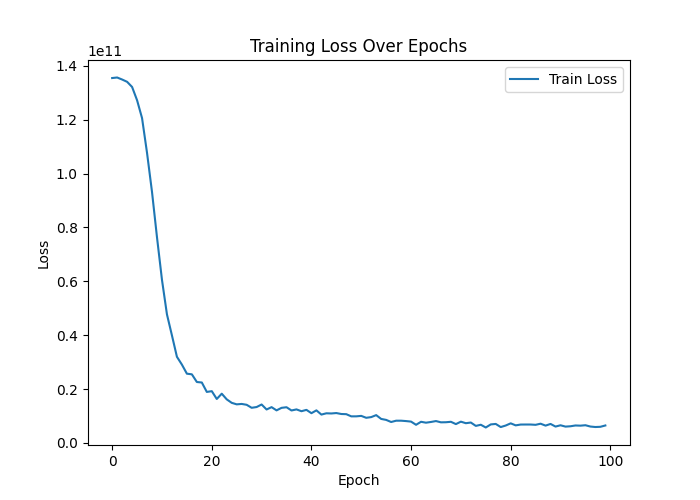
\includegraphics[width=1\linewidth]{training_loss.png}
    \caption{Training Loss}
    \label{fig:3}
\end{figure}

\subsection{Dataset Size and Splitting}
The complete dataset consisted of crop data spanning over the duration of 12 years (from 2010 to 2022), representing agricultural data over the level of countries over multiple years. The data was split as follows:

Training Set: 8 years (72\%)

Validation Set: 1 year (9\%)

Test Set: 2 years (18\%)

The training set was used to fit the model. The validation set was employed for monitoring training and tuning the hyper parameters of the model, and the test set was exclusively used for the final evaluation. This separation with these percentages ensured that the test performance is a reliable indicator of real world generalization.

The split was done chronologically, which is critical in time series forecasting to avoid leakage of future information into the model. This means that the model only had access to historical data when learning, closely mirroring its intended real world use.

\section{Model}
The core of the predictive framework is a multi layer perceptron (MLP), a class of artificial neural network renowned for its capacity to model complex non-linear relationships. The MLP was implemented using the PyTorch library. 

The architecture of the implemented MLP model is characterized by a sequence of interconnected layers: linear layers, ReLU activation functions, and dropout layers. Linear layers perform transformations on the input data, while ReLU activation functions introduce non-linearity, enabling the model to capture intricate patterns. Dropout layers, on the other hand, serve as a regularization technique to prevent over-fitting.

The model's performance is highly influenced by its hyper-parameters, which are parameters set prior to the training process. In this study, we meticulously optimized the following key hyper-parameters:

1. Learning Rate: The learning rate governs the step size the model takes to update its weights in response to the calculated error (loss). We explored learning rates of 0.0001 and 0.001 to find a balance between convergence speed and stability.

2. Hidden Layer Sizes: The hidden layers, situated between the input and output layers, are responsible for learning intermediate representations of the data. We experimented with two configurations: [64, 32, 16] and [128, 64], to assess the impact of network width and depth on performance.

3. Dropout Rate: Dropout is a regularization technique where neurons are randomly "dropped out" during training. We tested dropout rates of 0.2 and 0.3 to mitigate over-fitting.

4. Batch Size: The batch size determines the number of samples processed together in one iteration. We used batch sizes of 16 and 32 to evaluate computational efficiency and learning dynamics.

To identify the optimal combination of hyper-parameters, a grid search strategy was employed. This involved systematically evaluating the model's performance across all possible combinations of the specified hyper-parameter values.

After all the combination were tested, the following hyper-parameter values were selected based on the least RMSE value. The best batch size was 16, the best dropout percentage was 0.2, the best learning rate is 0.001, and the best hidden layer sizes is using 2 layers, input layer size is 64, first hidden layer size is 32, and the second hidden layer size is 16.

The model was trained using the Adam optimizer, an adaptive learning rate optimization algorithm that has demonstrated superior performance in various machine learning tasks. The Mean Squared Error (MSE) loss function was used to quantify the difference between the model's predictions and the actual values.

Over-fitting, a phenomenon where a model performs well on training data but poorly on unseen data, poses a significant challenge in machine learning. To mitigate over-fitting, two main methods were implemented. Firstly is integrating dropout layers into the model architecture to randomly deactivate neurons during training. This technique forces the network to learn redundant representations, enhancing its robustness and generalization. Secondly, the early stopping technique was used, early stopping monitors the model's performance on a validation set and halts the training process when the performance plateaus or starts to degrade. A patience of 10 epochs was set, in other words the training was stopped if the validation loss did not improve for 10 consecutive epochs.

\section{Features and Labels}
In the context of this study, the careful selection and extraction of features and labels are paramount to building a predictive model that accurately forecasts crop yield. The label, representing the target variable we aim to predict, and the features, representing the input variables used to make those predictions, form the foundation of our analysis.

The label used for training the model is total\_yield. This variable represents the total yield of crop products for a specific country in a given year. Crop yield is a critical indicator of agricultural productivity. Accurate forecasting of crop yield can provide valuable insights for policymakers, farmers, and other stakeholders, enabling them to make informed decisions and implement proactive strategies.

The features used as input to the model were carefully selected based on their potential relevance to crop yield and their statistical relationship with the label. The feature selection process involved several steps:

1. Correlation Analysis: the Pearson correlation coefficient was computed between each potential feature and the total\_yield label. The Pearson correlation coefficient measures the linear relationship between two variables, ranging from -1 (perfect negative correlation) to +1 (perfect positive correlation).

2. Thresholding: To identify the most relevant features, a threshold was set for the absolute value of the correlation coefficient. Features with an absolute correlation above this threshold were selected for inclusion in the model. This threshold was set to 0.3, indicating that we considered features with a moderate to strong linear relationship with crop yield.

3. Lagged Features: Recognizing the temporal nature of crop yield and its dependence on historical factors, lagged features was incorporated into the model. Lagged features are past values of the selected features, representing the influence of previous years' conditions on current crop yield. We included lags of up to two years for each selected feature, capturing the potential impact of short-term historical trends.

These were the selected features above the 0.3 threshold, the total yield, the standard deviation of the soil temp 10, the standard deviation of the soil temp 40, and the standard deviation of the soil temp 0. Then these features were lagged and inserted into the merged dataframe.

The rationale behind this feature selection approach is for a number of reasons:

- Relevance: By selecting features based on their correlation with the label, variables were prioritized that have a statistically significant relationship with crop yield. This helps to ensure that the model focuses on the most informative predictors, improving its accuracy and interpretability.

- Temporal Dynamics: Incorporating lagged features allows the model to capture the temporal dependencies in crop yield. Agricultural systems are influenced by factors that unfold over time, such as weather patterns, soil conditions, and agricultural practices. Lagged features enable the model to learn from these historical influences and make more accurate forecasts.

- Parsimony: Feature selection helps to reduce the dimensionality of the input space, leading to a more general model. A smaller number of features can improve the model's generalization performance, reduce the risk of over-fitting, and enhance computational efficiency.

In summary, the selection of total\_yield as the label and the careful extraction of relevant features, including lagged variables, were guided by the goal of building a robust and accurate model for forecasting crop yield. This approach leverages statistical analysis and domain knowledge to identify the most informative predictors and capture the temporal dynamics of agricultural systems.

\subsection{Lagged Features}
In order to ensure that only historically available information is used for prediction, lagged features were employed. Specifically, for each data instance at a certain year 't', the model input consisted of variables collected from the previous two years ('t-1' and 't-2'), while the target output was the yield at year 't'. This two-year lag preserves temporal causality and avoids data leakage.

One critical lagged feature is the crop yield of the previous year, which captures inertia and trends from recent growing seasons. In addition, features like soil temperature of different lengths, though recorded annually, were used in their t-th year form to predict the next year’s yield. This design reflects the realistic constraint that forecasts for year t+1 must rely entirely on information available up to year t and t-1.

By aligning features and labels in this manner, we constructed a dataset suitable for supervised learning that honours the temporal nature of agricultural systems.

\section{Preprocessing}
Before any preprocessing, all the 17 CSV files were merged together, some were merged using the 'inner' method and others were merged using the 'outer' method.

Data preprocessing is a vital step in any machine learning pipeline, particularly when dealing with real world data that may be incomplete, inconsistent, or unscaled. In this project, several preprocessing steps were applied to ensure data quality, consistency, and suitability for the MLP model.

Initially, the raw data contained missing values, in particular the soil moisture 100\_200 cm and the 'tws' comma-separated files, which can hinder the training process and introduce bias into the model. To address this, an interpolation technique to impute the missing values was employed. Specifically, a row wise interpolation across time series columns were performed. This method estimates missing values based on the values of neighbouring data points within the same row, preserving the temporal relationships within each data series.

During the data loading and merging phase, inconsistencies in the data structure across different files were encountered. Some files had different shapes or contained irrelevant information. To maintain consistency and focus on relevant data, certain files from the analysis was excluded from the first merge. These included files with different shapes, such as the country lookup file and land cover percentage data, as well as files with excessive missing values that were not suitable for interpolation. But they were merged later on in the second merge.

To prepare the categorical variable country for the MLP model, one-hot encoding was applied. One-hot encoding converts each category into a binary vector, where a value of 1 indicates the presence of that category and a value of 0 indicates its absence. This transformation allows the model to effectively process categorical information without imposing any ordinal relationship between categories.

Unlike the conventional train test split that is used to split the dataset randomly, which can cause leakage in time-series tasks, a chronological split was used to divide the data into training, validation, and test sets. This ensures that the model is only trained on past data and evaluated on future data, mimicking real deployment scenarios.

To ensure valid forecasting, input features from a certain year 't' were paired with yield labels from the previous two years ('t-1' and 't-2'). This required careful shifting of data to create aligned samples without leakage. Data from the the first two years was discarded since there were no past data beyond these two years.

Finally, to ensure that all features were on a comparable scale, feature scaling was applied using the standard scaler. Standard scaler standardises each feature by subtracting the mean and dividing by the standard deviation (z-score), resulting in features with zero mean and unit variance. Feature scaling is essential for neural network models, as it can improve convergence speed, prevent numerical instability, and ensure that all features contribute equally to the learning process.

These preprocessing steps were crucial for preparing the data for the MLP model, ensuring data quality, handling inconsistencies, and improving model performance.

\end{document}